\documentclass[12pt]{article}
\usepackage[utf8]{inputenc}
\usepackage{graphicx} % Allows you to insert figures
\usepackage{subcaption}
\usepackage{amsmath} % Allows you to do equations
\usepackage{fancyhdr} % Formats the header
\usepackage{geometry} % Formats the paper size, orientation, and margins
\usepackage{dirtytalk} % typesetting different types of quotation
\usepackage[english]{babel}
\usepackage{csquotes}
\usepackage{hyperref}
\usepackage{listings}
\usepackage{xcolor}
\usepackage{array}
\usepackage{caption}

% Define code style
\lstset{
  basicstyle=\ttfamily\small,
  backgroundcolor=\color{gray!10},
  frame=single,
  breaklines=true,
  postbreak=\mbox{\textcolor{red}{$\hookrightarrow$}\space},
  keywordstyle=\color{blue},
  commentstyle=\color{green!50!black},
  stringstyle=\color{orange},
}


\linespread{1.25} % About 1.5 spacing in Word
\setlength{\parindent}{0.8cm} % No paragraph indents
\setlength{\parskip}{0em} % Paragraphs separated by one line
\renewcommand{\headrulewidth}{0pt} % Removes line in header
\geometry{a4paper, portrait, margin=1in}
\setlength{\headheight}{14.49998pt}
\graphicspath{ {images/} }

\begin{document}
\begin{titlepage}
   \begin{center}
    \textsc{\large Ministry of Education of Republic of Moldova}\\[0.5cm]
    \textsc{\large Technical University of Moldova}\\[0.5cm]
    \textsc{\large Faculty of Computers, Informatics and Microelectronics}\\[0.5cm]
    \textsc{\large Department of Physics}\\[1.2cm]
    
    \vspace{25 mm}
    
    \textsc{\Large Criptography and security}\\[0.5cm]
    \textsc{\large Laboratory work \#2}\\[0.5cm]    % <<<<<<< CHANGE LAB NUMBER HERE
    
    \newcommand{\HRule}{\rule{\linewidth}{0.5mm}}
    \vspace{10 mm}
    \HRule \\[0.4cm]
    { \LARGE \bfseries Cryptanalysis of monoalphabetic ciphers.}\\[0.4cm] % <<<<<<< CHANGE LAB TITLE HERE
    \HRule \\[1.5cm]
    
    \vspace{10mm}
    
    \begin{minipage}[t]{0.4\textwidth}
    \begin{flushleft} \large
    \emph{Author:} \\
    Dmitrii \textsc{Belih}\\                         % <<<<<<< CHANGE YOUR NAME HERE
    std. gr. FAF-232                                % <<<<<<< CHANGE GROUP NUMBER HERE
    \end{flushleft}
    \end{minipage}
    ~
    \begin{minipage}[t]{0.4\textwidth}
    \begin{flushright} \large
    \emph{Verified:} \\
    \textsc{Zaica} M.\\
    \end{flushright}
    \end{minipage}\\[3cm]
    
    \vspace{5 mm}
    \large Chișinău 2025\\[0.5cm]
    
    \vfill
    \end{center}
\end{titlepage}

\setcounter{page}{2}
\pagestyle{fancy}
\fancyhf{}
\rhead{\thepage}
\lhead{FAF-232 Belih Dmitrii; Laboratory Work №2}




% \section*{Introduction}
\section*{Theory Background}
\hspace{0.8cm}

The weak point of monoalphabetic encryption systems lies in the frequency of appearance of characters in the text. If an encrypted text is long enough and the language in which the plaintext is written is known, the system can be broken by an attack based on the frequency of appearance of letters in a language (frequency analysis attack), this frequency being an intensively studied problem (not necessarily for cryptographic purposes) and as a result various ordering structures have been built relative to the frequency of appearance of letters in each European language and in other languages. Usually, the longer an encrypted text is, the closer the frequency of the letters used is to this general ordering. A comparison between the two ordering relationships (that of the characters in the encrypted text and that of the letters in the current language alphabet) leads to the realization of several correspondences (plaintext letter – ciphertext letter), which uniquely establishes the encryption key.
\begin{table}[h!]
    \centering
    \caption{Frecvența literelor limbii engleze}
    \label{tab:freq_eng}
    \begin{tabular}{|c|c|c|c|c|c|c|c|c|c|c|c|c|}
        \hline
        \textbf{A} & \textbf{B} & \textbf{C} & \textbf{D} & \textbf{E} & \textbf{F} & \textbf{G} & \textbf{H} & \textbf{I} & \textbf{J} & \textbf{K} & \textbf{L} & \textbf{M} \\
        \hline
        8.17 & 1.49 & 2.78 & 4.25 & 12.7 & 2.23 & 2.01 & 6.09 & 6.97 & 0.15 & 0.77 & 4.03 & 2.41 \\
        \hline
        \textbf{N} & \textbf{O} & \textbf{P} & \textbf{Q} & \textbf{R} & \textbf{S} & \textbf{T} & \textbf{U} & \textbf{V} & \textbf{W} & \textbf{X} & \textbf{Y} & \textbf{Z} \\
        \hline
        6.75 & 7.51 & 1.93 & 0.095 & 5.99 & 6.33 & 9.06 & 2.76 & 0.98 & 2.36 & 0.15 & 1.97 & 0.07 \\
        \hline
    \end{tabular}
    \parbox{\textwidth}{\small \textit{Pentru limba engleză avem situația prezentată în tabelul 2.2 și figura 2.2:}}
    \parbox{\textwidth}{\small \textit{Tabelul 2.2. Frecvența literelor limbii engleze}}
\end{table}
\begin{figure}[h!]
    \centering
    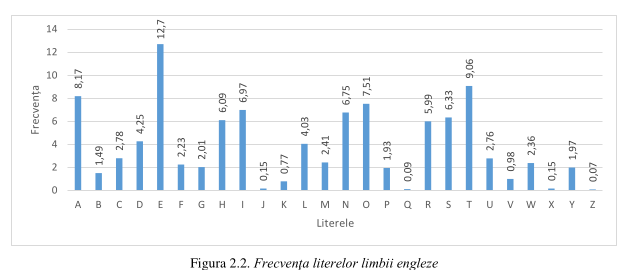
\includegraphics[width=0.8\textwidth]{img/Lom.png}
    \caption{Frequency of english letters}
    \label{fig:result1}
\end{figure}

\subsection*{Frequency analysis attack methodology}

We can use information about the frequency of letter occurrences in a language to attempt to break a monoalphabetic substitution cipher. This is possible because, for example, in a message written in English, the letter "E," which has the highest frequency, might be encrypted as "X." In that case, every "X" in the encrypted text would correspond to an "E" in the plaintext. Consequently, the most frequent letter in the encrypted text should be "X."

Thus, if we intercept an encrypted message and the most frequent letter in it is "P," we can assume that "P" was used to encrypt "E," and we can replace all "P"s with "E"s. Of course, not every text has exactly the same frequency, and as noted above, "T" and "A" also have high frequencies, so "P" could represent one of these. However, it is unlikely to be "Z," which is rarely encountered in English. By repeating this process with the next most frequent letter, we can make progress in breaking the message.

If we were to put all the letters in order and replace them according to the frequency table, it is most likely that we would not obtain the expected result. The cryptanalyst must use other "personality traits" of the letters to break the cryptogram. This may include examining pairs of letters (digraphs), the most common of which are TH, HE, AN, IN, ER, ON, RE, ED, ND, HA, AT, and EN. Triplets of letters (trigraphs) can also be very useful, with the most frequent in English being THE, AND, THA, ENT, ION, TIO, FOR, NDE, HAS, NCE, TIS, OFT, and MEN. Additionally, in English, only a few letters appear as doubles (SS, EE, TT, OO, and FF being the most frequent). There are only two meaningful single-letter words in English: "A" and "I."

Other frequent words also begin to emerge as we make some substitutions. For example, "T*E" may appear frequently after performing substitutions for "T" and "E." In this case, "T*E" is very likely to be "THE," a very common word in English.

The process of frequency analysis utilizes various subtle properties of the language, and for this reason, it is almost impossible for a computer to do all the work. Inevitably, a human element is necessary in this process to make informed decisions about which letters should be replaced.


\section*{The Task}

Either an encrypted message has been intercepted that is known to have been obtained using a monoalphabetic cipher. Applying the frequency analysis attack to find out the original message, assuming that it is a text written in English. Keep in mind that only the letters have been encrypted, the other characters remaining unencrypted.
\url{https://crypto.interactive-maths.com/frequency-analysis-breaking-the-code.html}

\textbf{My Variant: V2} \\
\textit{Wqv tooxwxng nc pvhivhf wn wqv witgpcniztwxngp uinodhvohifuwnjituqf. Widv, xw rtp zniv nc t
jtzv wqtg tgfwqxgj vspv—xw pndjqwwn ovstf hnzuivqvgpxng cni ngsf wqv pqniwvpw unppxasv
wxzv, gnw wqvsngjvpw—tgo wqv hifuwtgtsfpxp rtp, sxlvrxpv, edpw t udmmsv. Vjfuw'p rtpwqdp t
bdtpx hifuwnsnjf xg hngwitpw wn wqv ovtosf pvixndp phxvghv nc wnotf.Fvw jivtw wqxgjp qtkv
pztss avjxggxgjp, tgo wqvpv qxvinjsfuqp oxoxghsdov, wqndjq xg tg xzuvicvhw ctpqxng, wqv wrn
vsvzvgwp nc pvhivhf tgowitgpcniztwxng wqtw hnzuixpv wqv vppvgwxts twwixadwvp nc wqv
phxvghv. Tgopn hifuwnsnjf rtp anig. Xg xwp cxipw 3,000 fvtip, xw oxo gnw jinr pwvtoxsf.
Hifuwnsnjf tinpvxgovuvgovgwsf xg ztgf usthvp, tgo xg znpw nc wqvz xw oxvo wqv ovtwqp ncxwp
hxkxsxmtwxngp. Xg nwqvi usthvp, xw pdikxkvo, vzavoovo xg t sxwvitwdiv,tgo cinz wqxp wqvgvyw jvgvitwxng hndso hsxza wn qxjqvi svkvsp.Adw uinjivpp rtp psnr tgo evilf. Zniv rtp snpw wqtg
ivwtxgvo. Zdhq nc wqvqxpwnif nc hifuwnsnjf nc wqxp wxzv xp t utwhqrnil, t hitmf bdxsw
ncdgivstwvo xwvzp, puindwxgj, csndixpqxgj, rxwqvixgj. Ngsf wnrtio wqvRvpwvig Ivgtxpptghv
onvp wqv thhivwxgj lgnrsvojv avjxg wn adxso du tznzvgwdz. Wqv pwnif nc hifuwnsnjf odixgj
wqvpv fvtip xp, xg nwqvi rniop,vythwsf wqv pwnif nc ztglxgo. Hqxgt, wqv ngsf qxjq hxkxsxmtwxng
nc tgwxbdxwf wn dpv xovnjituqxhrixwxgj, pvvzp gvkvi wn qtkv ovkvsnuvo zdhq ivts hifuwnjituqf
—uviqtup cni wqtw ivtpng. Xg ngv htpv lgnrg cni zxsxwtif udiunpvp, wqv11wq-hvgwdif
hnzuxstwxng, Rd-hqxgj wpdgj-ftn ("Vppvgwxtsp cinz ZxsxwtifHstppxhp"), ivhnzzvgovo t widv xc
pztss hnov. Wn t sxpw nc 40 ustxgwvywxwvzp, itgjxgj cinz ivbdvpwp cni anrp tgo tiinrp wn wqv
ivuniw nc tkxhwnif, wqv hniivpungovgwp rndso tppxjg wqv cxipw 40 xovnjitzp nc tunvz. Wqvg,
rqvg t sxvdwvgtgw rxpqvo, cni vytzusv, wn ivbdvpw znivtiinrp, qv rtp wn Rixwv wqv hniivpungoxgj
xovnjitz tw t puvhxcxvo usthvng tg nioxgtif oxputwhq tgo pwtzu qxp pvts ng xw.Xg Hqxgt'p jivtw
gvxjqani wn wqv rvpw, Xgoxt, rqnpv hxkxsxmtwxngsxlvrxpv ovkvsnuvo vtisf tgo wn qxjq vpwtwv,
pvkvits cnizp nc pvhivwhnzzdgxhtwxngp rviv lgnrg tgo, t Uutivgwsf, uithwxhvo. Wqv Tiwqt-ptpwit,
t hstppxh rnil ng pwtwvhitcw twwixadwvo wn Ltdwxsft, xg ovphixaxgjwqv vpuxngtjv pvikxhv nc
Xgoxt tp uithwxhtssf ixoosxgj wqv hndgwif rxwqp Uxvp, ivhnzzvgovo wqtw wqv nccxhvip nc wqv
xgpwxwdwvp nc £ puxngtjv jxkvwqvxi puxvp wqvxi tppxjgzvgwp af pvhivw rixwxgj.Uviqtup znpw
xgwvivpwxgj wn hifuwnsnjxpwp, tztwvdi niuincvppxngts, xp wqtw Ktwpftftgt'p ctzndp wvywannl
nc vinwxhp, wqv Ltztpdwit,sxpwp pvhivw rixwxgj tp ngv nc wqv 64 tiwp, ni fnjtp, wqtw rnzvgpqndso
lgnr tgo uithwxhv. Wqv cndiwq jivtw hxkxsxmtwxng nc tgwxbdxwf, wqvZvpnun-wtzxtg, itwqvi
utitssvsvo Vjfuw vtisf xg xwp hifuwnjituqxhvknsdwxng, adw wqvg pdiutppvo xw. Wqdp, xg wqv
stpw uvixno nc hdgvxcnizrixwxgj, xg hnsnuqngp rixwwvg tw Didl (xg uivpvgw-otf Xitb) dgovi
wqvPvsvdhxo lxgjp xg wqv stpw cvr phniv fvtip avcniv wqv Hqixpwxtg vit,nhhtpxngts phixavp
hngkviwvo wqvxi gtzvp xgwn gdzavip. Wqvvghxuqvizvgw—xc pdhq xw av—ztf qtkv avvg ngsf cni
tzdpvzvgw ni wnpqnr ncc.}

\section*{Technical implementation}
\hspace{0.8cm}
First of all I need to analyze the frequency of letters in endlish text in my Variant. After using the provided tools I abserved this following photo
\begin{figure}[h!]
    \centering
    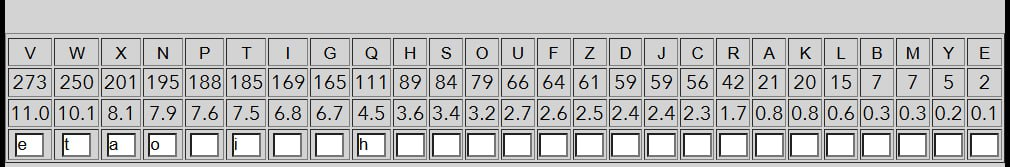
\includegraphics[width=0.8\textwidth]{img/Freq2.jpg}
    \label{fig:result1}
\end{figure}

Next step I can make comporision with the default frequency of english letter that wvreyone nows it. 

\begin{figure}[h!]
    \centering
    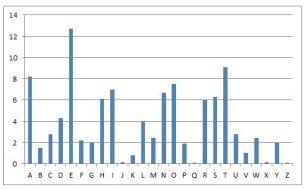
\includegraphics[width=0.8\textwidth]{img/def.png}
    \label{fig:result1}
\end{figure}

Now that we have all the letter frequencies in the ciphertext, we can start making some
substitutions. We see that the most frequent letter in the ciphertext is “V”, closely followed by “W”.
From the figure above, we can guess that these two letters represent “e” and
“t”, respectively, and after making these substitutions we get:

\textit{tQe TOOXtXNG NC PeHIeHF tN tQe tITGPCNIZTtXNGP UINODHeOHIFUtNJITUQF. tIDe, Xt RTP ZNIe NC T JTZe tQTG TGFtQXGJ eSPe—Xt PNDJQttN OeSTF HNZUIeQeGPXNG CNI NGSF tQe PQNItePt UNPPXASe tXZe, GNt tQeSNGJePt—TGO tQe HIFUtTGTSFPXP RTP, SXLeRXPe, EDPt T UDMMSe. eJFUt'P RTPtQDP T BDTPX HIFUtNSNJF XG HNGtITPt tN tQe OeTOSF PeIXNDP PHXeGHe NC tNOTF.Fet JIeTt tQXGJP QTKe PZTSS AeJXGGXGJP, TGO tQePe QXeINJSFUQP OXOXGHSDOe, tQNDJQ XG TG XZUeICeHt CTPQXNG, tQe tRN eSeZeGtP NC PeHIeHF TGOtITGPCNIZTtXNG tQTt HNZUIXPe tQe ePPeGtXTS TttIXADteP NC tQe PHXeGHe. TGOPN HIFUtNSNJF RTP ANIG. XG XtP CXIPt 3,000 FeTIP, Xt OXO GNt JINR PteTOXSF. HIFUtNSNJF TINPeXGOeUeGOeGtSF XG ZTGF USTHeP, TGO XG ZNPt NC tQeZ Xt OXeO tQe OeTtQP NCXtP HXKXSXMTtXNGP. XG NtQeI USTHeP, Xt PDIKXKeO, eZAeOOeO XG T SXteITtDIe,TGO CINZ tQXP tQe GeYt JeGeITtXNG HNDSO HSXZA tN QXJQeI SeKeSP.ADt UINJIePP RTP PSNR TGO EeILF. ZNIe RTP SNPt tQTG IetTXGeO. ZDHQ NC tQeQXPtNIF NC HIFUtNSNJF NC tQXP tXZe XP T UTtHQRNIL, T HITMF BDXSt NCDGIeSTteO XteZP, PUINDtXGJ, CSNDIXPQXGJ, RXtQeIXGJ. NGSF tNRTIO tQeRePteIG IeGTXPPTGHe ONeP tQe THHIetXGJ LGNRSeOJe AeJXG tN ADXSO DU TZNZeGtDZ. tQe PtNIF NC HIFUtNSNJF ODIXGJ tQePe FeTIP XP, XG NtQeI RNIOP,eYTHtSF tQe PtNIF NC ZTGLXGO. HQXGT, tQe NGSF QXJQ HXKXSXMTtXNG NC TGtXBDXtF tN DPe XOeNJITUQXHRIXtXGJ, PeeZP GeKeI tN QTKe OeKeSNUeO ZDHQ IeTS HIFUtNJITUQF —UeIQTUP CNI tQTt IeTPNG. XG NGe HTPe LGNRG CNI ZXSXtTIF UDIUNPeP, tQe11tQ-HeGtDIF HNZUXSTtXNG, RD-HQXGJ tPDGJ-FTN ("ePPeGtXTSP CINZ ZXSXtTIFHSTPPXHP"), IeHNZZeGOeO T tIDe XC PZTSS HNOe. tN T SXPt NC 40 USTXGteYtXteZP, ITGJXGJ CINZ IeBDePtP CNI ANRP TGO TIINRP tN tQe IeUNIt NC TKXHtNIF, tQe HNIIePUNGOeGtP RNDSO TPPXJG tQe CXIPt 40 XOeNJITZP NC TUNeZ. tQeG, RQeG T SXeDteGTGt RXPQeO, CNI eYTZUSe, tN IeBDePt ZNIeTIINRP, Qe RTP tN RIXte tQe HNIIePUNGOXGJ XOeNJITZ Tt T PUeHXCXeO USTHeNG TG NIOXGTIF OXPUTtHQ TGO PtTZU QXP PeTS NG Xt.XG HQXGT'P JIeTt GeXJQANI tN tQe RePt, XGOXT, RQNPe HXKXSXMTtXNGSXLeRXPe OeKeSNUeO eTISF TGO tN QXJQ ePtTte, PeKeITS CNIZP NC PeHIetHNZZDGXHTtXNGP ReIe LGNRG TGO, T UUTIeGtSF, UITHtXHeO. tQe TItQT-PTPtIT, T HSTPPXH RNIL NG PtTteHITCt TttIXADteO tN LTDtXSFT, XG OePHIXAXGJtQe ePUXNGTJe PeIKXHe NC XGOXT TP UITHtXHTSSF IXOOSXGJ tQe HNDGtIF RXtQP UXeP, IeHNZZeGOeO tQTt tQe NCCXHeIP NC tQe XGPtXtDteP NC £ PUXNGTJe JXKetQeXI PUXeP tQeXI TPPXJGZeGtP AF PeHIet RIXtXGJ.UeIQTUP ZNPt XGteIePtXGJ tN HIFUtNSNJXPtP, TZTteDI NIUINCePPXNGTS, XP tQTt KTtPFTFTGT'P CTZNDP teYtANNL NC eINtXHP, tQe LTZTPDtIT,SXPtP PeHIet RIXtXGJ TP NGe NC tQe 64 TItP, NI FNJTP, tQTt RNZeGPQNDSO LGNR TGO UITHtXHe. tQe CNDItQ JIeTt HXKXSXMTtXNG NC TGtXBDXtF, tQeZePNUN-tTZXTG, ITtQeI UTITSSeSeO eJFUt eTISF XG XtP HIFUtNJITUQXHeKNSDtXNG, ADt tQeG PDIUTPPeO Xt. tQDP, XG tQe STPt UeIXNO NC HDGeXCNIZRIXtXGJ, XG HNSNUQNGP RIXtteG Tt DIDL (XG UIePeGt-OTF XITB) DGOeI tQePeSeDHXO LXGJP XG tQe STPt CeR PHNIe FeTIP AeCNIe tQe HQIXPtXTG eIT,NHHTPXNGTS PHIXAeP HNGKeIteO tQeXI GTZeP XGtN GDZAeIP. tQeeGHXUQeIZeGt—XC PDHQ Xt Ae—ZTF QTKe AeeG NGSF CNI TZDPeZeGt NI tNPQNR NCC
}

Next step is define the comon words so whe famous word is THE and we can see that where is the similar words like this. 
We now notice that the word "tQe" appears frequently in the passage. In English, the most common how I say 3-letter word is "the" and this fits with what we have already done, which suggests that the "Q" should be deciphered to "h".

And we have following text now:
\textit{the TOOXtXNG NC PeHIeHF tN the tITGPCNIZTtXNGP UINODHeOHIFUtNJITUhF. tIDe, Xt RTP ZNIe NC T JTZe thTG TGFthXGJ eSPe—Xt PNDJhttN OeSTF HNZUIeheGPXNG CNI NGSF the PhNItePt UNPPXASe tXZe, GNt theSNGJePt—TGO the HIFUtTGTSFPXP RTP, SXLeRXPe, EDPt T UDMMSe. eJFUt'P RTPthDP T BDTPX HIFUtNSNJF XG HNGtITPt tN the OeTOSF PeIXNDP PHXeGHe NC tNOTF.Fet JIeTt thXGJP hTKe PZTSS AeJXGGXGJP, TGO thePe hXeINJSFUhP OXOXGHSDOe, thNDJh XG TG XZUeICeHt CTPhXNG, the tRN eSeZeGtP NC PeHIeHF TGOtITGPCNIZTtXNG thTt HNZUIXPe the ePPeGtXTS TttIXADteP NC the PHXeGHe. TGOPN HIFUtNSNJF RTP ANIG. XG XtP CXIPt 3,000 FeTIP, Xt OXO GNt JINR PteTOXSF. HIFUtNSNJF TINPeXGOeUeGOeGtSF XG ZTGF USTHeP, TGO XG ZNPt NC theZ Xt OXeO the OeTthP NCXtP HXKXSXMTtXNGP. XG NtheI USTHeP, Xt PDIKXKeO, eZAeOOeO XG T SXteITtDIe,TGO CINZ thXP the GeYt JeGeITtXNG HNDSO HSXZA tN hXJheI SeKeSP.ADt UINJIePP RTP PSNR TGO EeILF. ZNIe RTP SNPt thTG IetTXGeO. ZDHh NC thehXPtNIF NC HIFUtNSNJF NC thXP tXZe XP T UTtHhRNIL, T HITMF BDXSt NCDGIeSTteO XteZP, PUINDtXGJ, CSNDIXPhXGJ, RXtheIXGJ. NGSF tNRTIO theRePteIG IeGTXPPTGHe ONeP the THHIetXGJ LGNRSeOJe AeJXG tN ADXSO DU TZNZeGtDZ. the PtNIF NC HIFUtNSNJF ODIXGJ thePe FeTIP XP, XG NtheI RNIOP,eYTHtSF the PtNIF NC ZTGLXGO. HhXGT, the NGSF hXJh HXKXSXMTtXNG NC TGtXBDXtF tN DPe XOeNJITUhXHRIXtXGJ, PeeZP GeKeI tN hTKe OeKeSNUeO ZDHh IeTS HIFUtNJITUhF —UeIhTUP CNI thTt IeTPNG. XG NGe HTPe LGNRG CNI ZXSXtTIF UDIUNPeP, the11th-HeGtDIF HNZUXSTtXNG, RD-HhXGJ tPDGJ-FTN ("ePPeGtXTSP CINZ ZXSXtTIFHSTPPXHP"), IeHNZZeGOeO T tIDe XC PZTSS HNOe. tN T SXPt NC 40 USTXGteYtXteZP, ITGJXGJ CINZ IeBDePtP CNI ANRP TGO TIINRP tN the IeUNIt NC TKXHtNIF, the HNIIePUNGOeGtP RNDSO TPPXJG the CXIPt 40 XOeNJITZP NC TUNeZ. theG, RheG T SXeDteGTGt RXPheO, CNI eYTZUSe, tN IeBDePt ZNIeTIINRP, he RTP tN RIXte the HNIIePUNGOXGJ XOeNJITZ Tt T PUeHXCXeO USTHeNG TG NIOXGTIF OXPUTtHh TGO PtTZU hXP PeTS NG Xt.XG HhXGT'P JIeTt GeXJhANI tN the RePt, XGOXT, RhNPe HXKXSXMTtXNGSXLeRXPe OeKeSNUeO eTISF TGO tN hXJh ePtTte, PeKeITS CNIZP NC PeHIetHNZZDGXHTtXNGP ReIe LGNRG TGO, T UUTIeGtSF, UITHtXHeO. the TIthT-PTPtIT, T HSTPPXH RNIL NG PtTteHITCt TttIXADteO tN LTDtXSFT, XG OePHIXAXGJthe ePUXNGTJe PeIKXHe NC XGOXT TP UITHtXHTSSF IXOOSXGJ the HNDGtIF RXthP UXeP, IeHNZZeGOeO thTt the NCCXHeIP NC the XGPtXtDteP NC £ PUXNGTJe JXKetheXI PUXeP theXI TPPXJGZeGtP AF PeHIet RIXtXGJ.UeIhTUP ZNPt XGteIePtXGJ tN HIFUtNSNJXPtP, TZTteDI NIUINCePPXNGTS, XP thTt KTtPFTFTGT'P CTZNDP teYtANNL NC eINtXHP, the LTZTPDtIT,SXPtP PeHIet RIXtXGJ TP NGe NC the 64 TItP, NI FNJTP, thTt RNZeGPhNDSO LGNR TGO UITHtXHe. the CNDIth JIeTt HXKXSXMTtXNG NC TGtXBDXtF, theZePNUN-tTZXTG, ITtheI UTITSSeSeO eJFUt eTISF XG XtP HIFUtNJITUhXHeKNSDtXNG, ADt theG PDIUTPPeO Xt. thDP, XG the STPt UeIXNO NC HDGeXCNIZRIXtXGJ, XG HNSNUhNGP RIXtteG Tt DIDL (XG UIePeGt-OTF XITB) DGOeI thePeSeDHXO LXGJP XG the STPt CeR PHNIe FeTIP AeCNIe the HhIXPtXTG eIT,NHHTPXNGTS PHIXAeP HNGKeIteO theXI GTZeP XGtN GDZAeIP. theeGHXUheIZeGt—XC PDHh Xt Ae—ZTF hTKe AeeG NGSF CNI TZDPeZeGt NI tNPhNR NCC
}
tN = to 
Xt  = it 
\section*{Results}
\hspace{0.8cm}

\textit{Task1}

\begin{figure}[h!]
    \centering
    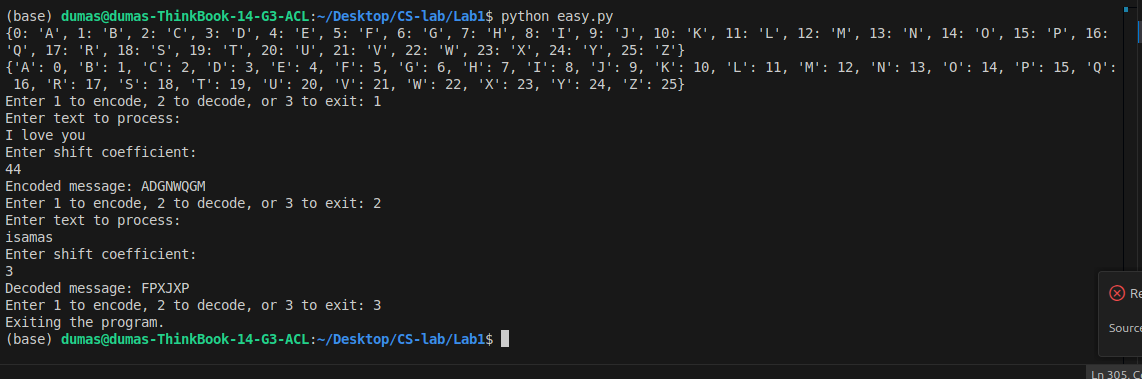
\includegraphics[width=0.8\textwidth]{img/Res1.png}
    \caption{Result of the encoding and decoding program}
    \label{fig:result1}
\end{figure}

\textit{Task2}

\begin{figure}[h!]
    \centering
    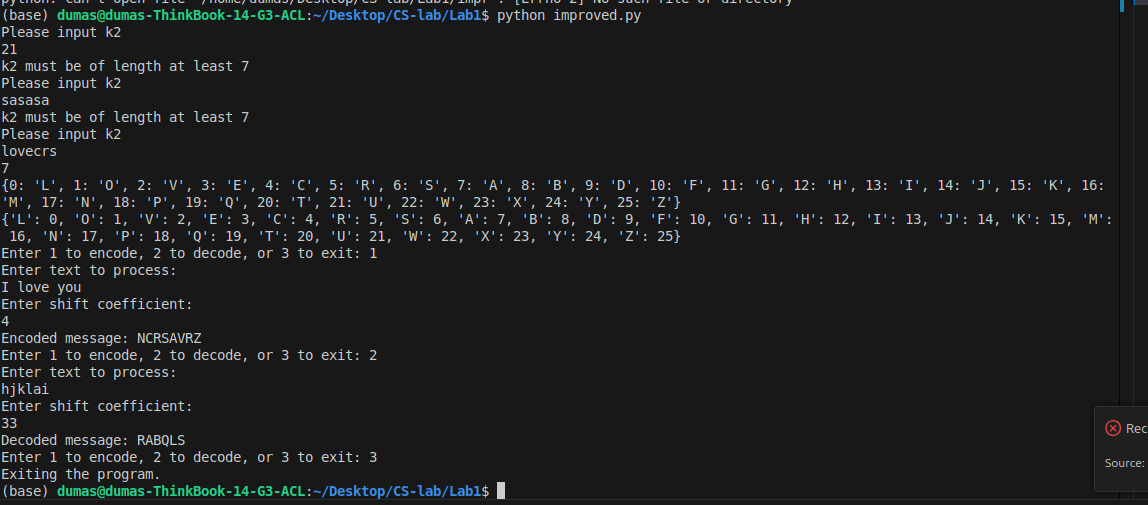
\includegraphics[width=0.8\textwidth]{img/Res2.png}
    \caption{Result of the encoding and decoding program}
    \label{fig:result1}
\end{figure}





\section*{Conclusion}
\hspace{0.8cm}

In this laboratory work, we explored the fundamentals of classical cryptography through the implementation of the Caesar cipher and its enhanced version with a keyword-based alphabet permutation. The Caesar cipher, a simple substitution cipher, was implemented to perform encryption and decryption by shifting letters in the English alphabet by a user-defined key \( k_1 \), adhering to the formulas \( E_{k_1}(x) = (x + k_1) \mod 26 \) and \( D_{k_1}(y) = (y - k_1) \mod 26 \). The program for Task 1 successfully handled user inputs, ensuring that only valid alphabetic characters and key values between 1 and 25 were processed, with text converted to uppercase and spaces removed for consistency.

For Task 2, we extended the Caesar cipher by incorporating a second key, \( k_2 \), which reordered the alphabet based on a user-provided keyword of at least seven letters. This permutation increased the cipher's complexity by altering the standard alphabet order before applying the Caesar shift. The implementation ensured robust input validation, rejecting non-alphabetic characters in the keyword and maintaining a unique letter mapping for the custom alphabet. Both tasks were implemented in Python, providing an interactive interface for encoding and decoding messages while demonstrating the practical application of modular arithmetic in cryptography.

The results of both implementations, as shown in the provided figures, confirmed the correctness of the encryption and decryption processes. The programs successfully transformed input texts into their corresponding ciphertexts and back, maintaining fidelity to the theoretical framework. This laboratory work highlighted the strengths and limitations of the Caesar cipher, particularly its vulnerability to brute-force attacks due to a small key space in the basic version, and how a keyword-based permutation can enhance its security.

Overall, this exercise provided valuable insights into the principles of classical ciphers, the importance of input validation in secure programming, and the role of modular arithmetic in cryptographic transformations. It also underscored the trade-offs between simplicity and security in cryptographic systems, laying a foundation for understanding more complex encryption methods.


% \section*{Bibliography}
% \hspace{0.8cm}
% \begin{enumerate}
%   \item Resource 1
%   \item Resource 2
%   \item Resource 3 
% \end{enumerate}

\pagebreak
\end{document}